\documentclass[11pt]{beamer}
\usetheme{Warsaw}
\usepackage[utf8]{inputenc}
\usepackage[polish]{babel}
\usepackage{amsmath}
\usepackage{amsfonts}
\usepackage{amssymb}
\usepackage{graphicx}
\usepackage{polski}
\renewcommand*{\figurename}{Rys.}
\usepackage{float}
\usepackage{geometry}
\usepackage{listings}

\author{Marek Grudkowski \\ Kamil Kaczmarkiewicz}
\title{Światowy program szczepień \\ przeciwko COVID-19}
\subtitle{Eksploracja Danych}
%\setbeamercovered{transparent} 
%\setbeamertemplate{navigation symbols}{} 

\institute{Politechnika Gdańska} 
\date{}
\subject{} 
\begin{document}

\begin{frame}
\titlepage
\end{frame}


\begin{frame}{Ogólny opis danych}
\begin{itemize}
\item zbiór danych opisujący postęp światowego programu szczepień przeciwko COVID-19
\item celem eksploracji w głównej mierze jest odnalezienie jak najlepszej strategii dla państw biorących udział w programie szczepień
\item dane pochodzą z wielu źródeł, którymi są organy krajowe lub lokalne
\item zbiór aktualnie zawiera ponad $13300$ przykładów, ale co kilka dni jest aktualizowany
\item jeden przykład jest opisany za pomocą 15 atrybutów
\end{itemize}
\end{frame}

\begin{frame}{Opis atrybutów nominalnych}
\begin{itemize}
\item \textbf{country} - nazwa regionu lub państwa, z którego pochodzą dane
\item \textbf{ISO code} - trzyliterowy kod państwa zgodny z normą  ISO 3166-1
\item \textbf{date} - data pozyskania danych
\item \textbf{source name} - nazwa organu z którego pochodzą dane
\item \textbf{source website} - strona internetowa, z której pobrano dane
\end{itemize}
\end{frame}

\begin{frame}{Opis atrybutów numerycznych}
\begin{itemize}
	\item \textbf{total vaccinations} - całkowita, sumaryczna liczba podanych dawek w danym kraju
	\item \textbf{total vaccinations per hundred} - powyższy atrybut, ale w przeliczeniu na stu mieszkańców
	\item \textbf{people vaccinated} - całkowita, sumaryczna liczba osób w dany kraju, która przyjęła choć jedną dawkę szczepionki
	\item \textbf{people vaccinated per hundred} - powyższy atrybut, ale w przeliczeniu na stu mieszkańców
\end{itemize}
\end{frame}

\begin{frame}{Opis atrybutów numerycznych}
\begin{itemize}
	\item \textbf{people fully vaccinated} - całkowita, sumaryczna liczba osób w dany kraju, które są w pełni zaszczepione
	\item \textbf{people fully vaccinated per hundred} - powyższy atrybut, ale w przeliczeniu na stu mieszkańców
	\item \textbf{daily vaccinations} - całkowita, sumaryczna liczba podanych dawek w danym kraju w ciągu dnia, liczba ta jest wygładzana w ujęciu 7 dni
	\item \textbf{daily vaccinations per milion} - powyższy atrybut, ale w przeliczeniu na milion mieszkańców
	\item \textbf{daily vaccinations raw} - dzienna zmiana w całkowitej liczbie podanych dawek, surowy środek wykorzystywany przy kontroli danych, autorzy zbioru nie zalecają korzystania z tego atrybutu podczas analizy
\end{itemize}
\end{frame}

\begin{frame}[fragile]{Analiza atrybutów nominalnych} 
\begin{itemize}
\item część kodów ISO nie jest zapisana wedle standardu (są to regiony leżące w obrębie różnych państw)
\item można takie przykłady zaktualizować
\item wówczas należy sprawdzić, czy dla danego państwa nie ma więcej niż 1 przykładu dla jednej daty
\end{itemize}
\begin{lstlisting}
England has code OWID_ENG
Kosovo has code OWID_KOS
Northern Cyprus has code OWID_CYN
Northern Ireland has code OWID_NIR
Scotland has code OWID_SCT
Wales has code OWID_WLS
\end{lstlisting}
\end{frame}


% wykres pudełkowy pokazujący ilość przykładów per państwo

\begin{frame}
\begin{figure}[h]
\centering
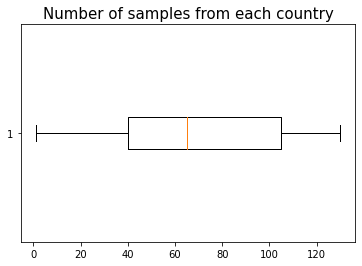
\includegraphics[scale=0.5]{../img/boxplot_of_samples.png} 
\caption{Liczba przykładów dostarczonych przez poszczególne państwa}
\label{Rys:boxplotSamples}
\end{figure}
\end{frame}

% histogram pokazujący ilość przykładów per państwo

\begin{frame}
\begin{figure}[h]
\centering
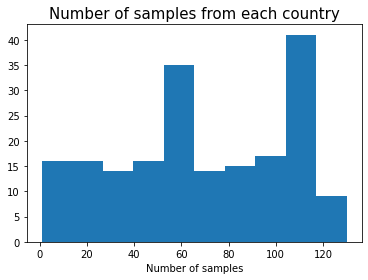
\includegraphics[scale=0.5]{../img/number_of_samples.png} 
\caption{Liczba przykładów dostarczonych przez poszczególne państwa}
\label{Rys:histogramSamples}
\end{figure}
\end{frame}

% opis korelacji atrybutów numerycznych

\begin{frame}
\begin{itemize}
\item atrybuty numeryczne można połączyć w pary \textit{wartość bezwzględna} i \textit{wartość względna}
\item takie pary cechują się korelacją równą jeden
\item \textbf{daily vaccinations raw} nie analizujemy, gdyż autorzy nie zalecają korzystania z tego atrybutu
\end{itemize}
\end{frame}

% korelacja pomiędzy atrybutami dla całego zbioru

\begin{frame}{Korelacja między atrybutami dla całego zbioru}
\begin{figure}
\centering
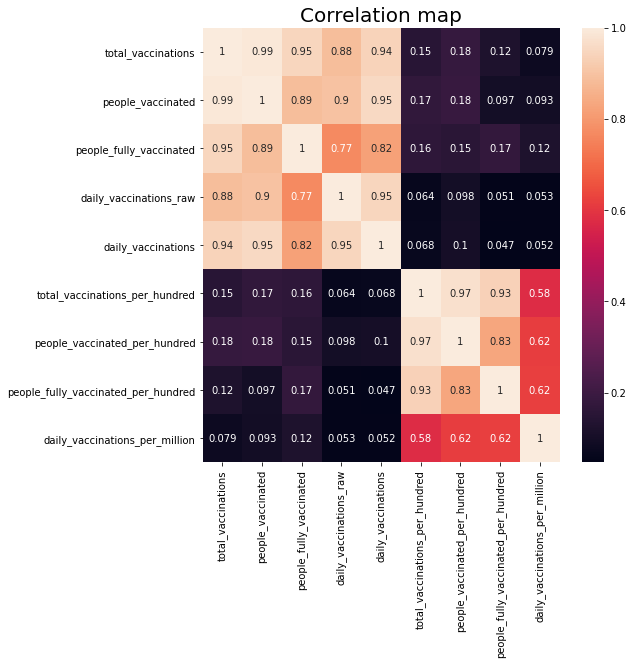
\includegraphics[scale=0.4]{../img/corelation.png} 
\caption{Korelacja pomiędzy atrybutami całego zbioru danych\label{Rys:corrHeatMapWorld}}
\end{figure}
\end{frame}

% korelacja pomiędzy atrybutami per państwo

\begin{frame}{Korelacja między atrybutami podzielona na państwa}
\begin{figure}
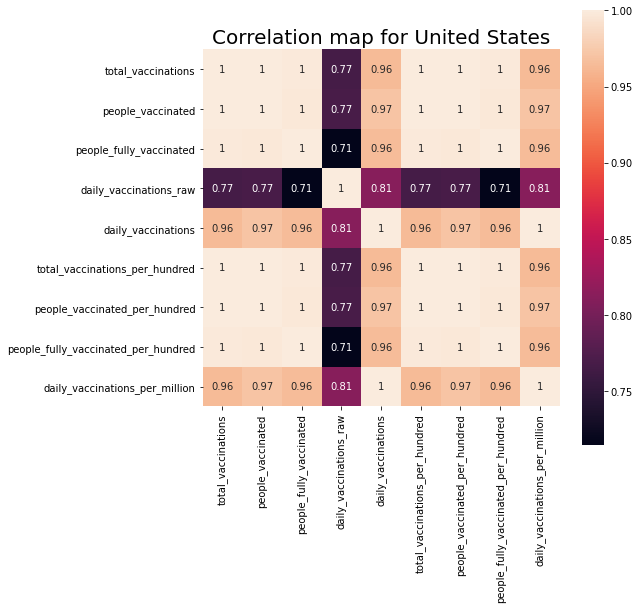
\includegraphics[scale=0.4]{../img/usa_corr.png} 
\caption{Korelacja pomiędzy atrybutami zbioru danych dla USA}
\label{Rys:corrHeatMapUsa}
\end{figure}
\end{frame}

% brakujące wartości w zbiorze danych

\begin{frame}[fragile]{Brakujące wartości}
\begin{lstlisting}
Size of data is: (13307, 13)
Missing values in dataset: 
country                                   0
iso_code                                  0
date                                      0
total_vaccinations                     5255
people_vaccinated                      5931
people_fully_vaccinated                7926
daily_vaccinations_raw                 6529
daily_vaccinations                      220
total_vaccinations_per_hundred         5255
people_vaccinated_per_hundred          5931
people_fully_vaccinated_per_hundred    7926
daily_vaccinations_per_million          220
vaccines                                  0
\end{lstlisting}
\end{frame}

% opis atrybutów numerycznych

\begin{frame}
\begin{itemize}
	\item część z brakujących wartości można łatwo uzupełnić, wykorzystując zależności między atrybutami
	\item przykładowo łączną sumę podanych dawek szczepionki można wyznaczyć prostą metodą, jeśli założymy liniową progresją pomiędzy odległymi wartościami
	\item trochę inaczej wygląda sytuacja w przypadku dziennej ilości podanych dawek. Według autorów zbioru danych jest to atrybut, który obliczają sami według procedury
	\begin{itemize}
\begin{small}
		\item Za pomocą interpolacji uzupełnia się brakujące wartości totalnej liczby wykonanych szczepień
		\item Na podstawie różnicy z dniem poprzednim wylicza się ilość podanych w danym dniu dawek
		\item Taka wyliczona liczba jest ostatecznie uśredniana z wartością jaka występuje w ciągu ostatniego tygodnia 
\end{small}
	\end{itemize}
\end{itemize}
\end{frame}

% wykres pudełkowy 1  

\begin{frame}
\begin{figure}[!ht]
\centering
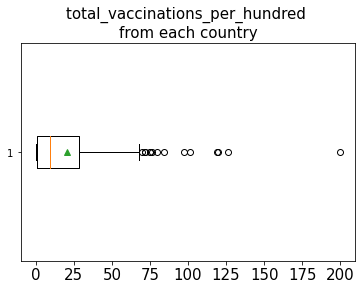
\includegraphics[scale=0.5]{../img/box_total_vaccinations.png} 
\caption{Rozkład liczby wykonanych szczepień}
\label{Rys:boxTotalVacc}
\end{figure}
\end{frame}

% wykres pudełkowy 2  

\begin{frame}
\begin{figure}[!ht]
\centering
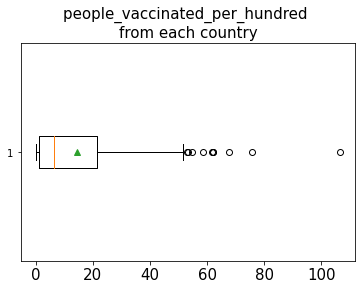
\includegraphics[scale=0.5]{../img/box_people_vaccinated.png} 
\caption{Rozkład liczby zaszczepionych osób}
\label{Rys:boxPeopleVacc}
\end{figure}
\end{frame}

% wykres pudełkowy 3
 
\begin{frame}
\begin{figure}[h]
\centering
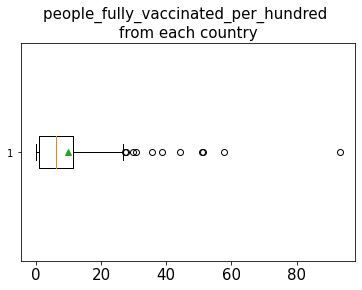
\includegraphics[scale=0.5]{../img/box_fully_vaccinated.png} 
\caption{Rozkład liczby w pełni zaszczepionych osób}
\label{Rys:boxFullyVacc}
\end{figure}
\end{frame}

% podsumowanie

\begin{frame}{Wnioski z EAD}
\begin{itemize}
\item wady to duża rozbieżność ilości przykładów na państwo oraz duże braki w wartościach atrybutów
\item rozkłady wartości atrybutów zapewniają tutaj dużo informacji i pokazują ogólny postęp programu szczepień
\item dużą zaletą jest to, że dane są aktualizowane na bieżąco
\item podsumowując, cele określone na początku wymagają odpowiedniego przygotowania danych, ale są możliwe do realizacji
\end{itemize}
\end{frame}

\end{document}